\chapter{Literature Review and Related Work}
\label{chap:relatedworks}

\section{Competitor Analysis}
\label{section:competitor-analysis}

The competitive landscape for fitness technology is currently divided between manual tracking applications and high-cost industrial hardware. Prometheus positions itself as an automated, non-intrusive solution that leverages existing infrastructure to provide high-utility data at a lower entry cost for facility owners.

\begin{figure}[h]
    \centering
    % Note: Replace 'example-image' with your actual file name
    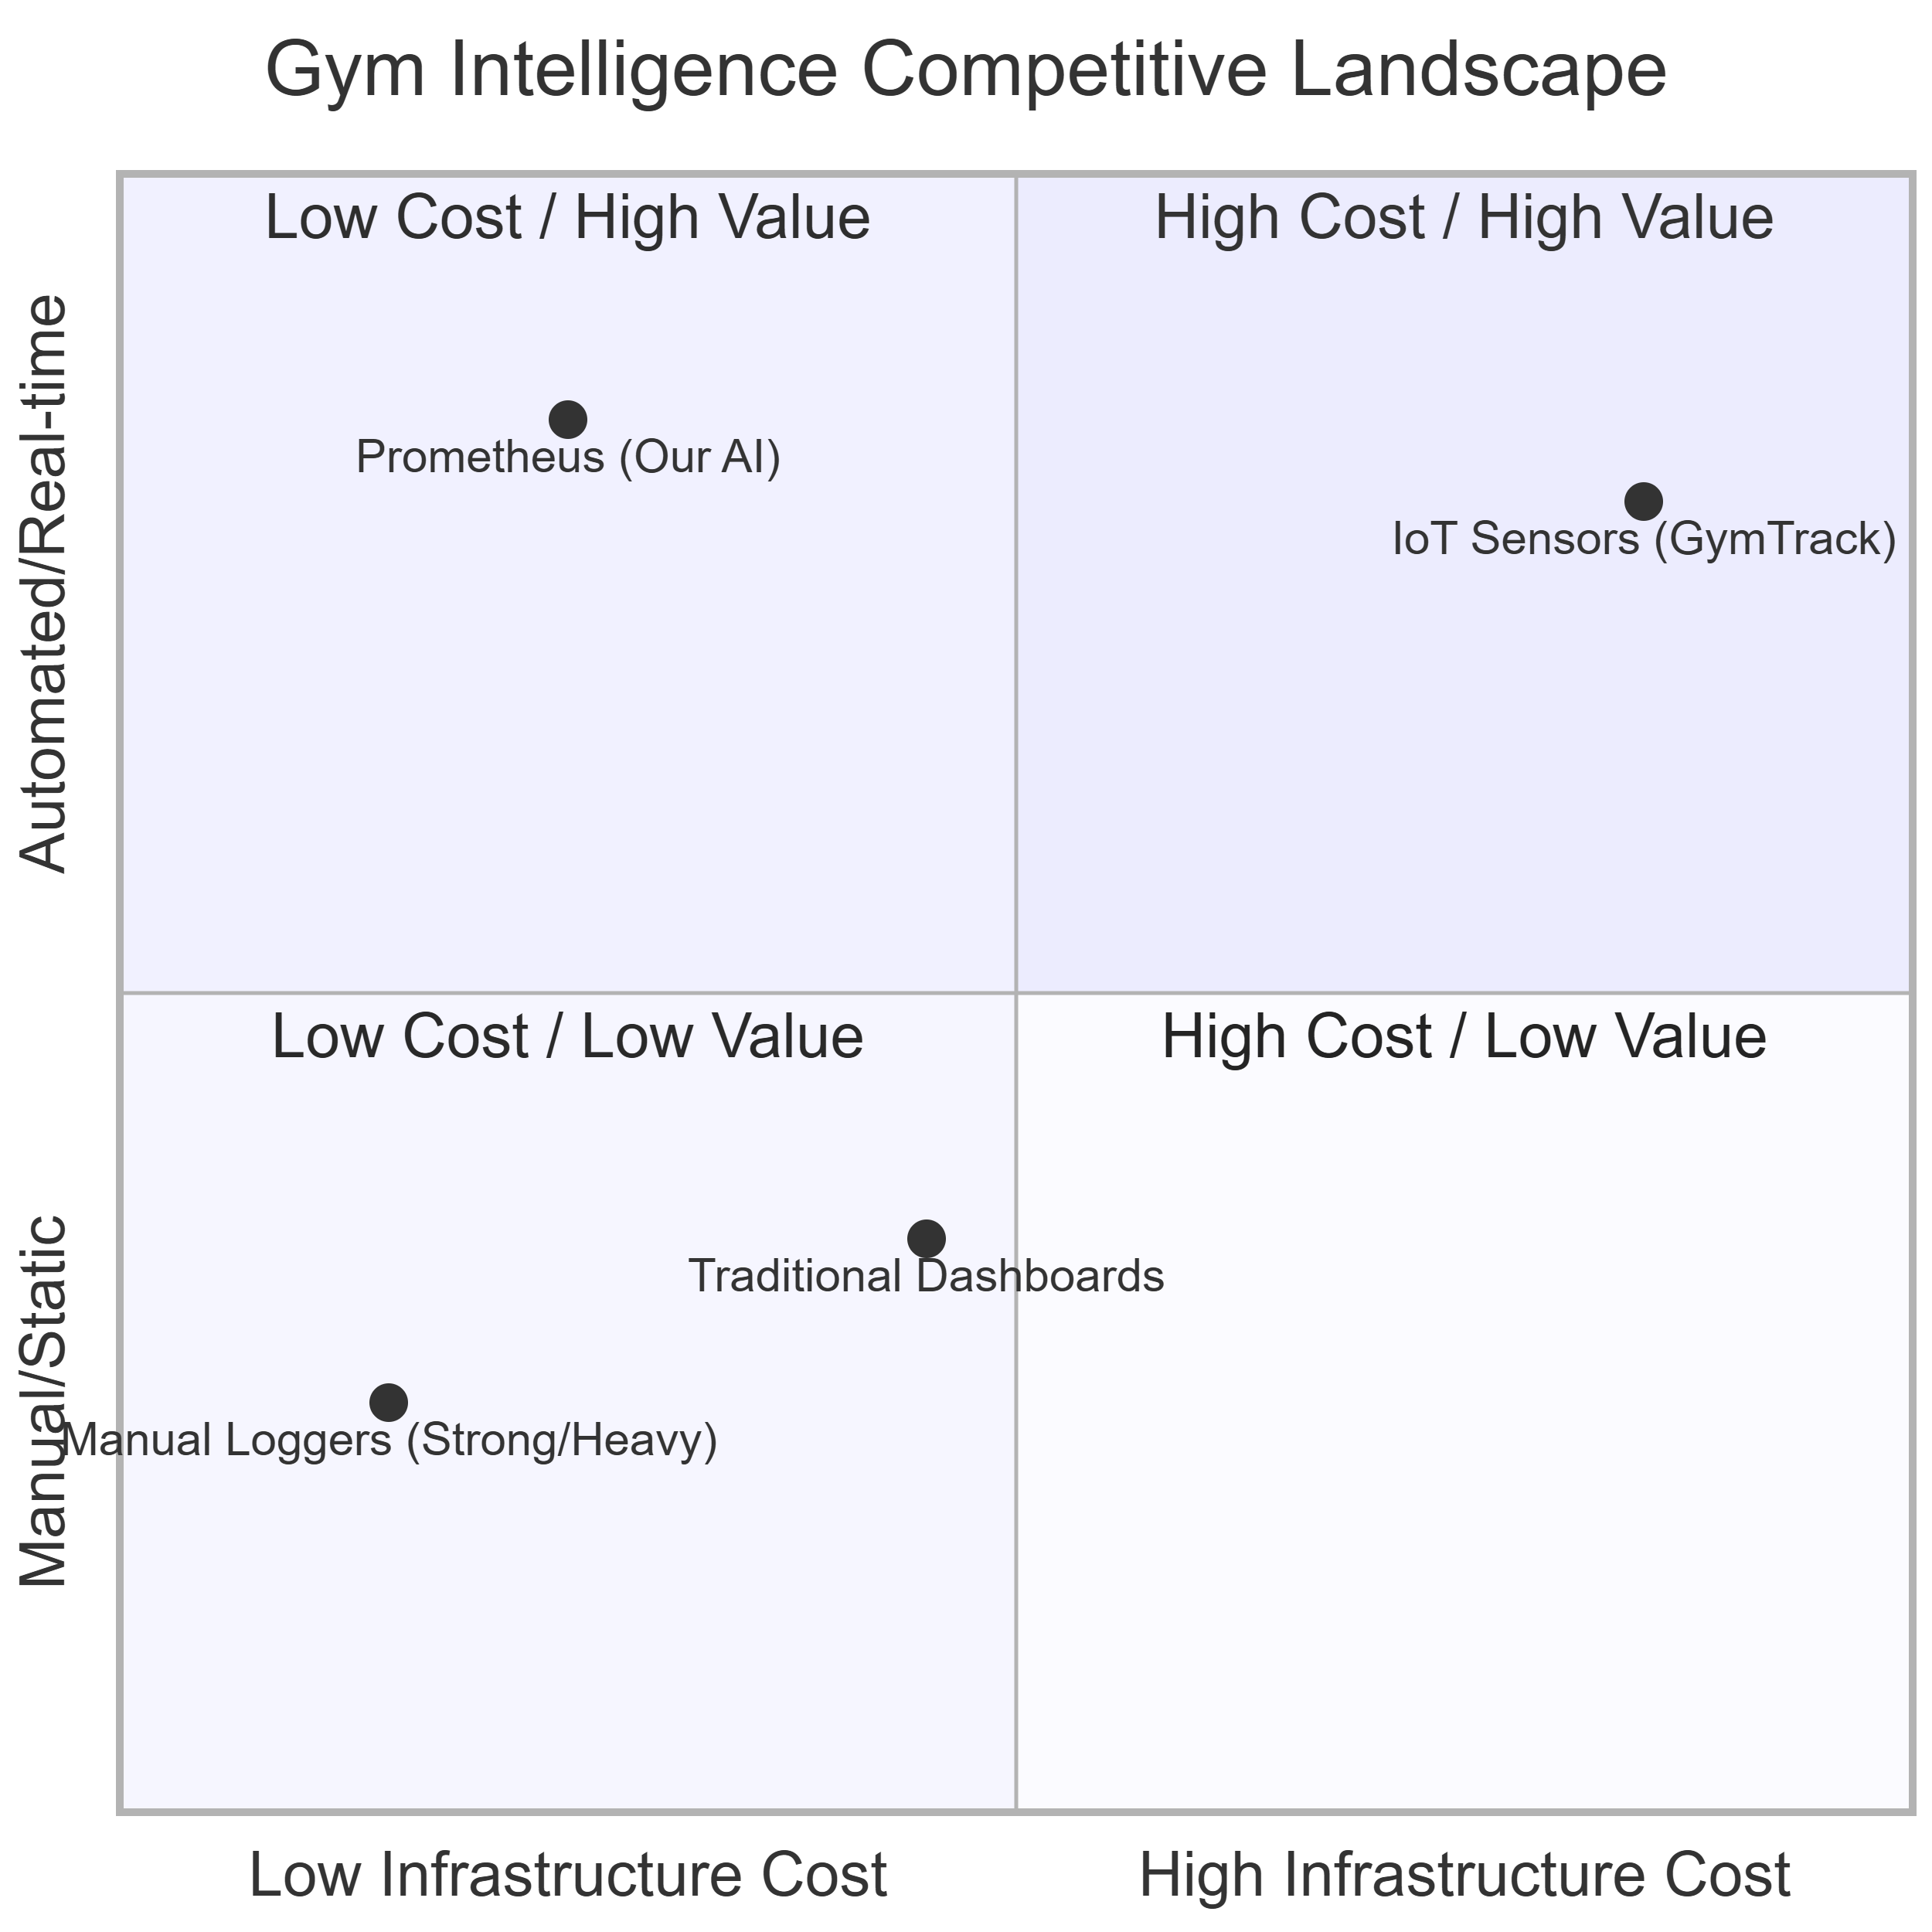
\includegraphics[width=0.8\textwidth]{assets/figures/Competitor.png} 
    \caption{Competitive Landscape: Automation vs. Infrastructure Cost}
    \label{fig:competitor-landscape}
\end{figure}

The following table provides a detailed comparison between Prometheus and existing solutions in the market, highlighting the gaps in real-time spatial intelligence.

\begin{table}[h]
\centering
\footnotesize % Reduces font size (can also use \small or \scriptsize)
\renewcommand{\arraystretch}{1.5} % Increases row height for better readability
\setlength{\tabcolsep}{4pt} % Reduces horizontal padding between columns

\begin{tabularx}{\textwidth}{|l|X|X|X|X|}
\hline
\textbf{Feature} & \textbf{Prometheus} & \textbf{Manual Loggers} & \textbf{IoT Sensors} & \textbf{Gym Dashboards} \\ \hline
Real-time Occupancy & Automated & None & Automated & Manual Entry \\ \hline
Installation Cost & Low (CCTV) & Zero & High (Per-unit) & Moderate \\ \hline
Member Utility & High & High & Low & Moderate \\ \hline
Spatial Analytics & Heatmaps & None & Numeric Only & Attendance Only \\ \hline
Privacy & Edge-based & High & High & Moderate \\ \hline
\end{tabularx}
\caption{Comparison Table of Competitive Fitness Solutions}
\label{table:competitor-analysis}
\end{table}

\section{Literature Review}
\label{section:literature-review}

To build a technically sound and feasible system, this project draws from several key academic works and technical advancements in the fields of Computer Vision and Distributed Systems.

\subsection{Real-Time Object Detection (YOLO Architecture)}
The foundation of the occupancy detection engine is based on the "You Only Look Once" (YOLO) architecture. Research by Redmon et al. established that frame-rate inference is possible by treating detection as a single regression problem. This project specifically evaluates the use of YOLOv8 and YOLOv10. The selection of YOLOv10 informs our choice for edge deployment, as its elimination of Non-Maximum Suppression (NMS) significantly reduces computational latency on local hardware.

\subsection{Vision-Based Gym Monitoring (GymCam)}
The "GymCam" project by Khurana et al. demonstrated the viability of using unconstrained camera feeds to track multiple users and exercises simultaneously. Their research indicates that while fine-grained action recognition is complex, identifying machine occupancy through spatial overlap is highly reliable. Prometheus extends this logic by utilizing a multi-camera RTSP network to provide floor-wide spatial analytics.

\subsection{Large-Scale Multi-View Datasets (M3GYM)}
For model training, this project utilizes the M3GYM dataset. Unlike standard datasets, M3GYM provides multi-view labels in real-world gym environments characterized by high occlusion. This informs the design of our "Occupancy Logic," allowing the system to distinguish between a person walking near equipment and a person actively utilizing a machine.

\subsection{Privacy-Preserving Edge Computing}
A primary constraint for gym-based AI is member privacy (GDPR/PDPA). Current literature suggests that performing inference at the "edge" allows raw video data to be discarded immediately after metadata extraction. This informs our choice of an Edge Processing Layer (e.g., ASUS NUC), ensuring that no identifiable video frames are ever transmitted to the cloud.